\section{Observation and Calculations}

\begin{enumerate}

\item \textbf{Astable Multivibrator}
\begin{enumerate}
    \item \textbf{With duty cycle more than 50\%}
        \begin{itemize}
            \item $R_A=9.87$ \kohm, $R_B=9.75$ \kohm
            \item $C_T=10.30$ nF
        \end{itemize}

        \begin{table}[H]
            \centering
            \begin{tabular}{|c|c|c|c|}\hline
                Parameter & Theoretical & Observed & Error \\ 
                          & Value       & Value    &       \\ \hline 
                $f_\text{osc}$   & 492.3 $\pm$ 0.6 Hz & 490.2 Hz & $-0.3\%$  \\ \hline
                Duty Cycle       & 66.80 $\pm$ 0.02 \% & 66.7\%  & $-0.1\%$ \\ \hline
            \end{tabular}
            % \caption{Observed and Theoretical Values}
        \end{table}

    \begin{figure}[H]
        \centering
        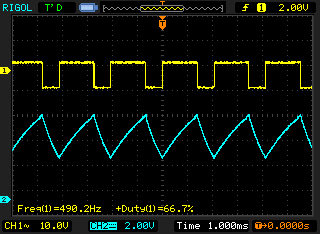
\includegraphics[width=0.80\columnwidth]{images/astable1.png}
        \caption{Oscilloscope output of an astable multivibrator (above) with duty cycle 66.7\% and the voltage across $C_T$ (below)}
        % \label{fig:0}
    \end{figure}

    \item \textbf{With duty cycle less than 50\%}
        \begin{itemize}
            \item $R_A=2.844$ \kohm, $R_B=9.75$ \kohm
            \item $C_T=10.3$ nF
        \end{itemize}

        \begin{table}[H]
            \centering
            \begin{tabular}{|c|c|c|c|}\hline
                Parameter & Theoretical & Observed & Error \\ 
                        & Value       & Value    &       \\ \hline 
                $f_\text{osc}$   & 1.148 $\pm$ 0.002 kHz & 1.020 kHz & $-12.5\%$  \\ \hline
                Duty Cycle       & 22.58 $\pm$ 0.06 \% & 22.4\%  & $-0.8\%$ \\ \hline
            \end{tabular}
            % \caption{Observed and Theoretical Values}
        \end{table}

        \begin{figure}[H]
            \centering
            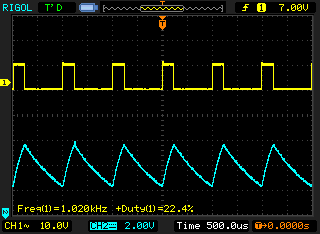
\includegraphics[width=0.80\columnwidth]{images/astable2.png}
            \caption{Oscilloscope output of an astable multivibrator (above) with duty cycle 22.4\% and the voltage across $C_T$ (below)}
            % \label{fig:0}
        \end{figure}

    \item \textbf{With variable duty cycle from 0 to 100\%}
        \begin{itemize}
            \item $R_1=0.975$ \kohm, $R_3=2.844$ \kohm
            \item $R_X=10.19$ \kohm
            \item $C_T=10.3$ nF
            \item Theoretical $f_\text{osc}=2.150 \pm 0.005$ kHz
        \end{itemize}

        \subsubsection*{Oscilloscope Outputs}

        \begin{figure}[H]
            \centering
            \begin{subfigure}[b]{0.4\textwidth}
                \centering
                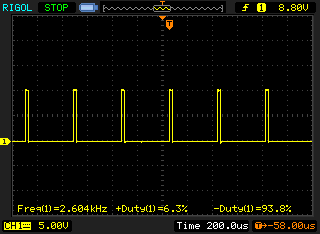
\includegraphics[width=\textwidth]{images/astable31.png}
                \caption{Duty cycle $= 6.3\%$ and $f_\text{osc}=2.604$ kHz}
            \end{subfigure}
            \hfill
            \begin{subfigure}[b]{0.4\textwidth}
                \centering
                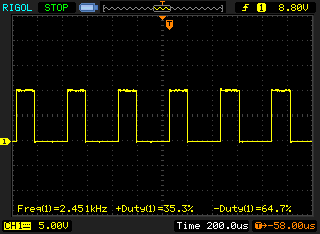
\includegraphics[width=\textwidth]{images/astable32.png}
                \caption{Duty cycle $= 35.3\%$ and $f_\text{osc}=2.451$ kHz}
            \end{subfigure}
            \hfill
            % \begin{subfigure}[b]{0.4\textwidth}
            %     \centering
            %     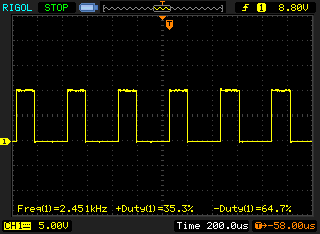
\includegraphics[width=\textwidth]{images/astable32.png}
            %     \cap-tion{Duty cycle $= 35.3\%$ and $f_\text{osc}=2.451$ kHz}
            % \end{subfigure}
            % \hfill
            \begin{subfigure}[b]{0.4\textwidth}
                \centering
                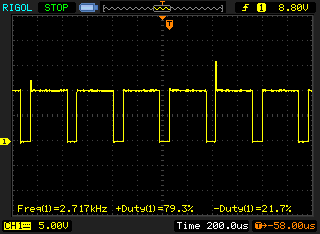
\includegraphics[width=\textwidth]{images/astable34.png}
                \caption{Duty cycle $= 79.3\%$ and $f_\text{osc}=2.717$ kHz}
            \end{subfigure}
            \hfill
            \caption{Oscilloscope outputs of an astable multivibrator with variable duty cycle}
       \end{figure}

        \begin{table}[H]
            \centering
            \begin{tabular}{|c|c|c|c|c|c|}\hline
                $R_A$ & $R_B$ & Observed & \multicolumn{2}{c|}{Duty Cycle (\%)} & Error \\ \cline{4-5}
                (\kohm) & (\kohm) & $f_\text{osc}$ (kHz) & Observed & Theoretical & \\ \hline        
                0.978 & 12.984& 2.604 & 6.3  & 6.97 $\pm$ 0.01  & $ -9.6\%$\\ \hline
                5.541 & 8.784 & 2.451 & 35.3 & 39.55 $\pm$ 0.08 &  $-10.7\%$\\ \hline
                7.585 & 6.647 & 2.525 & 51.5 & 54.14 $\pm$ 0.08 & $ -4.9\%$\\ \hline
                11.11 & 2.846 & 2.717 & 79.3 & 79.69 $\pm$ 0.09 & $ -0.3\%$\\ \hline
                
            \end{tabular}
            % \caption{Observed and Theoretical Values}
        \end{table}

        % \begin{itemize}
            \noindent Minimum duty cycle = $6.3\%$\\
            Maximum duty cycle = $79.3\%$\\
            Avg. $f_\text{osc}$ = $(2.574 \pm 0.114) $ kHz\\\\
        % \end{itemize}
       

\end{enumerate}

\item \textbf{Monostable Multivibrator}\\

    \begin{itemize}
        \item $R=99.7$ \kohm, $C=96\,\mu$F
        \item Pulse width (Output High Duration):
            \begin{itemize}
                \item Observed: 10.96 s
                \item Calculated: (10.53 $\pm$ 0.02) s
                \item Error: $3.9\%$
            \end{itemize}
    \end{itemize}

    \begin{figure}[H]
        \centering
        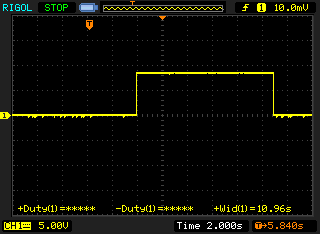
\includegraphics[width=1\columnwidth]{images/monostable.png}
        \caption{Oscilloscope output of a monostable multivibrator with pulse width $=10.96$ s}
        % \label{fig:0}
    \end{figure}

\item \textbf{Bistable Multivibrator}\\\\
According to Fig. \ref{bis2}, F refers to the \verb|TrIGGER| pin which is used output the \verb|SET| state and and G refers to the \verb|THRESHOLD| which is used to get the \verb|RESET| state.
\begin{table}[H]
    \centering
    \begin{tabular}{|c|c|c|}\hline
        Point & Connected to & Output \\ \hline
        F & Ground   & SET \\ \hline
        G & $V_{CC}$ & RESET  \\ \hline
    \end{tabular}
    % \caption{Observed and Theoretical Values}
\end{table}
\begin{figure}[H]
    \centering
    \begin{subfigure}[b]{0.45\textwidth}
        \centering
        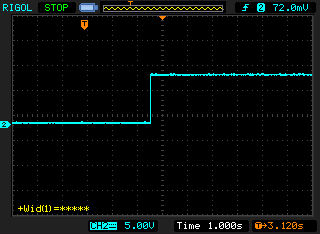
\includegraphics[width=\textwidth]{images/bi2.png}
        \caption{}
    \end{subfigure}
    \hfill
    \begin{subfigure}[b]{0.45\textwidth}
        \centering
        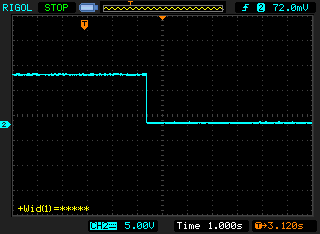
\includegraphics[width=\textwidth]{images/bi4.png}
        \caption{}
    \end{subfigure}
    \hfill
    \caption{Oscilloscope outputs of a bistable multivibrator for (a) SET condition and (b) RESET condition}
\end{figure}


\end{enumerate}